\section{Model predictions errors for provinces in Vietnam}

% ERRORS

\begin{landscape}
\begin{table}[!htb]
    \centering
    \begin{tabular}{| c | c | c | c | c | c | c | c | c | c | c |}
        \multirow{2}{*}{Days}
            & \multirow{2}{*}{Loc.}
            & \multicolumn{3}{c |}{Baseline}
            & \multicolumn{3}{c |}{2nd. Version}
            & \multicolumn{3}{c |}{3rd. Version} \\ \cline{3-11}
            & & MAE & MAPE & RMSE & MAE & MAPE & RMSE & MAE & MAPE & RMSE \\ \hline\hline

        \multirow{4}{*}{7}
            & Binh Duong & \textbf{95.426} & \textbf{5.812} & \textbf{98.695} & 100.100 & 6.106 & 102.736 & 121.271 & 7.385 & 125.535 \\
            & Dong Nai & \textbf{70.096} & \textbf{16.939} & \textbf{70.288} & 94.131 & 22.727 & 94.283 & 77.339 & 18.677 & 77.493 \\
            & Ho Chi Minh city & \textbf{969.400} & \textbf{35.439} & \textbf{991.778} & 976.721 & 35.690 & 999.832 & 1015.894 & 37.060 & 1042.086 \\
            & Long An & 94.571 & 33.788 & 95.339 & \textbf{8.248} & \textbf{2.931} & \textbf{8.550} & 61.189 & 21.732 & 63.484 \\ \hline

        \multirow{4}{*}{14}
            & Binh Duong & 139.067 & 7.795 & 147.809 & \textbf{138.019} & \textbf{7.764} & \textbf{144.724} & 176.025 & 9.869 & 186.921 \\
            & Dong Nai & \textbf{59.087} & \textbf{13.976} & \textbf{60.270} & 87.745 & 20.673 & 88.071 & 70.580 & 16.639 & 71.003 \\
            & Ho Chi Minh city & \textbf{1403.959} & \textbf{38.084} & \textbf{1489.430} & 1423.473 & 38.555 & 1512.527 & 1515.313 & 40.813 & 1619.890 \\
            & Long An & 115.136 & 38.395 & 117.520 & \textbf{11.775} & \textbf{3.890} & \textbf{12.432} & 92.512 & 30.445 & 99.238 \\ \hline

        \multirow{4}{*}{21}
            & Binh Duong & 177.847 & 9.335 & 190.719 & \textbf{168.792} & \textbf{8.910} & \textbf{177.966} & 223.925 & 11.759 & 239.736 \\
            & Dong Nai & \textbf{55.633} & \textbf{12.716} & \textbf{56.685} & 87.775 & 19.906 & 87.995 & 72.183 & 16.345 & 72.517 \\
            & Ho Chi Minh city & \textbf{1891.890} & \textbf{40.052} & \textbf{2062.596} & 1926.393 & 40.695 & 2104.055 & 2095.582 & 43.845 & 2309.499 \\
            & Long An & 134.235 & 42.112 & 138.380 & \textbf{14.507} & \textbf{4.507} & \textbf{15.372} & 124.800 & 38.414 & 136.510 \\ \hline

        \multirow{4}{*}{28}
            & Binh Duong & 203.904 & 10.232 & 217.207 & \textbf{185.288} & \textbf{9.373} & \textbf{193.737} & 257.546 & 12.925 & 274.293 \\
            & Dong Nai & \textbf{52.644} & \textbf{11.686} & \textbf{53.744} & 87.106 & 19.115 & 87.288 & 74.530 & 16.270 & 74.884 \\
            & Ho Chi Minh city & \textbf{2387.155} & \textbf{41.454} & \textbf{2637.652} & 2434.133 & 42.186 & 2693.007 & 2701.371 & 46.196 & 3022.084 \\
            & Long An & 151.608 & 45.047 & 157.341 & \textbf{16.404} & \textbf{4.841} & \textbf{17.303} & 157.136 & 45.593 & 173.810 \\ \hline
    \end{tabular}
    \caption{Out-of-sample errors of the model's predictions on the number of deaths for the provinces in Vietnam. The lowest errors for each evaluation metrics at each location are highlighted.}
\end{table}
\end{landscape}

\begin{landscape}
\begin{table}[!htb]
    \centering
    \begin{tabular}{| c | c | c | c | c | c | c | c | c | c | c |}
        \multirow{2}{*}{Days}
            & \multirow{2}{*}{Loc.}
            & \multicolumn{3}{c |}{Baseline}
            & \multicolumn{3}{c |}{2nd. Version}
            & \multicolumn{3}{c |}{3rd. Version} \\ \cline{3-11}
            & & MAE & MAPE & RMSE & MAE & MAPE & RMSE & MAE & MAPE & RMSE \\
        \hline\hline

        \multirow{4}{*}{7}
            & Binh Duong & 258.212 & 8.744 & 299.194 & \textbf{116.056} & \textbf{4.086} & \textbf{164.898} & 296.040 & 9.960 & 330.132 \\
            & Dong Nai & 130.533 & 17.341 & 135.187 & 209.730 & 27.792 & 214.491 & \textbf{39.442} & \textbf{5.266} & \textbf{49.236} \\
            & Ho Chi Minh city & \textbf{139.151} & \textbf{3.560} & \textbf{163.295} & 376.279 & 9.647 & 394.165 & 705.167 & 18.114 & 723.858 \\
            & Long An & 189.861 & 33.532 & 200.279 & 188.479 & 33.290 & 198.773 & \textbf{157.530} & \textbf{27.707} & \textbf{168.869} \\ \hline

        \multirow{4}{*}{14}
            & Binh Duong & 508.485 & 16.627 & 597.647 & \textbf{205.217} & \textbf{6.720} & \textbf{267.533} & 545.052 & 17.835 & 626.841 \\
            & Dong Nai & \textbf{84.028} & \textbf{11.122} & \textbf{103.395} & 179.143 & 23.323 & 186.383 & 133.415 & 16.778 & 169.034 \\
            & Ho Chi Minh city & \textbf{379.416} & \textbf{9.804} & \textbf{466.377} & 600.225 & 15.498 & 651.818 & 989.250 & 25.554 & 1040.354 \\
            & Long An & 199.785 & 36.232 & 211.350 & 197.566 & 35.802 & 209.171 & \textbf{163.229} & \textbf{29.231} & \textbf{176.954} \\ \hline

        \multirow{4}{*}{21}
            & Binh Duong & 514.164 & 25.439 & 596.107 & \textbf{500.765} & 32.829 & 695.279 & 518.767 & \textbf{24.589} & \textbf{594.628} \\
            & Dong Nai & \textbf{63.199} & \textbf{8.373} & \textbf{85.472} & 173.204 & 22.846 & 178.936 & 174.459 & 22.671 & 202.875 \\
            & Ho Chi Minh city & \textbf{742.775} & \textbf{17.905} & \textbf{960.595} & 902.403 & 22.027 & 1040.717 & 1338.583 & 32.902 & 1468.122 \\
            & Long An & 153.175 & 30.224 & 176.074 & 150.502 & 29.573 & 173.932 & \textbf{112.808} & \textbf{20.656} & \textbf{144.752} \\ \hline

        \multirow{4}{*}{28}
            & Binh Duong & 650.869 & 59.526 & 741.151 & 787.829 & 87.134 & 1021.467 & \textbf{623.044} & \textbf{54.074} & \textbf{696.459} \\
            & Dong Nai & \textbf{51.988} & \textbf{7.033} & \textbf{74.758} & 177.252 & 24.773 & 181.688 & 179.379 & 24.798 & 200.903 \\
            & Ho Chi Minh city & \textbf{1297.598} & \textbf{27.166} & 1713.583 & 1388.426 & 29.725 & \textbf{1697.844} & 1863.602 & 40.654 & 2149.100 \\
            & Long An & 118.454 & 24.197 & 152.753 & 116.804 & 23.893 & 150.918 & \textbf{98.185} & \textbf{21.637} & \textbf{128.612} \\ \hline
    \end{tabular}
    \caption{Out-of-sample errors of the model's predictions on the number of new cases for the provinces in Vietnam. The lowest errors for each evaluation metrics at each location are highlighted.}
\end{table}
\end{landscape}

\begin{landscape}
\begin{table}[!htb]
    \centering
    \begin{tabular}{| c | c | c | c | c | c | c | c | c | c | c |}
        \multirow{2}{*}{Days}
            & \multirow{2}{*}{Loc.}
            & \multicolumn{3}{c |}{Baseline}
            & \multicolumn{3}{c |}{2nd. Version}
            & \multicolumn{3}{c |}{3rd. Version} \\ \cline{3-11}
            & & MAE & MAPE & RMSE & MAE & MAPE & RMSE & MAE & MAPE & RMSE \\ \hline\hline

        \multirow{4}{*}{7}
            & Binh Duong & \textbf{543.123} & \textbf{0.300} & \textbf{669.448} & 1080.846 & 0.605 & 1092.888 & 2716.160 & 1.539 & 2807.759 \\
            & Dong Nai & 925.781 & 2.478 & 968.738 & 1151.564 & 3.071 & 1239.187 & \textbf{171.280} & \textbf{0.473} & \textbf{191.766} \\
            & Ho Chi Minh city & 2880.532 & 2.432 & 2897.982 & \textbf{1146.135} & \textbf{0.998} & \textbf{1337.867} & 1530.084 & 1.231 & 1929.637 \\
            & Long An & 1838.836 & 8.607 & 1885.619 & 558.175 & 2.541 & 694.931 & \textbf{358.230} & \textbf{1.733} & \textbf{408.240} \\ \hline

        \multirow{4}{*}{14}
            & Binh Duong & 2672.053 & 1.341 & 3614.244 & \textbf{834.983} & \textbf{0.450} & \textbf{894.195} & 2511.522 & 1.337 & 2752.084 \\
            & Dong Nai & 1216.773 & 3.022 & 1267.355 & 1809.578 & 4.441 & 1961.363 & \textbf{538.527} & \textbf{1.284} & \textbf{749.337} \\
            & Ho Chi Minh city & \textbf{2038.919} & \textbf{1.623} & \textbf{2269.591} & 2365.506 & 1.693 & 2975.292 & 5096.246 & 3.529 & 6552.386 \\
            & Long An & 2689.645 & 11.316 & 2851.355 & 1400.049 & 5.699 & 1684.345 & \textbf{791.856} & \textbf{3.278} & \textbf{942.779} \\ \hline

        \multirow{4}{*}{21}
            & Binh Duong & 3647.509 & 1.764 & 4430.807 & \textbf{1576.284} & \textbf{0.770} & \textbf{2335.074} & 2776.520 & 1.406 & 3008.196 \\
            & Dong Nai & \textbf{1278.627} & 2.994 & \textbf{1314.002} & 2364.315 & 5.378 & 2573.613 & 1282.437 & \textbf{2.779} & 1737.311 \\
            & Ho Chi Minh city & \textbf{3863.159} & \textbf{2.489} & \textbf{5067.508} & 5495.625 & 3.348 & 7444.975 & 10170.384 & 6.199 & 13131.423 \\
            & Long An & 3228.181 & 12.685 & 3406.408 & 1927.496 & 7.360 & 2204.703 & \textbf{1084.391} & \textbf{4.180} & \textbf{1233.620} \\ \hline

        \multirow{4}{*}{28}
            & Binh Duong & 3212.031 & 1.538 & 3992.435 & 4506.591 & 2.075 & 7143.902 & \textbf{2646.462} & \textbf{1.308} & \textbf{2953.921} \\
            & Dong Nai & \textbf{1307.494} & \textbf{2.909} & \textbf{1334.511} & 2948.022 & 6.268 & 3243.385 & 2048.294 & 4.150 & 2650.432 \\
            & Ho Chi Minh city & \textbf{8875.541} & \textbf{4.700} & \textbf{13108.589} & 11039.327 & 5.797 & 15550.166 & 17695.850 & 9.442 & 23398.714 \\
            & Long An & 3549.776 & 13.298 & 3714.577 & 2237.386 & 8.175 & 2480.566 & \textbf{1193.084} & \textbf{4.410} & \textbf{1312.184} \\ \hline
    \end{tabular}
    \caption{Out-of-sample errors of the model's predictions on the number of cumulative cases for the provinces in Vietnam. The lowest errors for each evaluation metrics at each location are highlighted.}
\end{table}
\end{landscape}

\subsection{Reproduction number and fatality rate}

\begin{figure}[!htb]
    \centering

    \begin{subfigure}[b]{\linewidth}
        \centering
        \begin{subfigure}[b]{0.4\linewidth}
            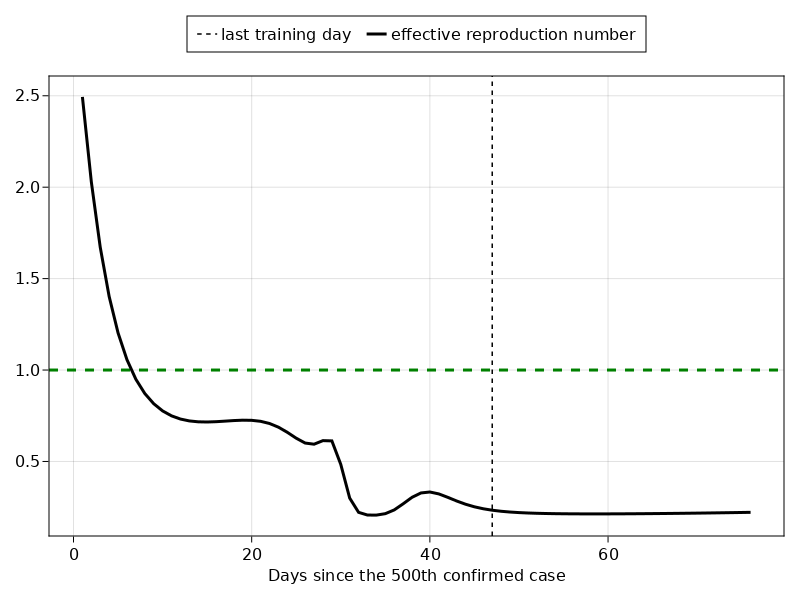
\includegraphics[width=\linewidth]{baseline/binhduong/20211216111951.baseline.binhduong.R_effective.png}
        \end{subfigure}
        \begin{subfigure}[b]{0.4\linewidth}
            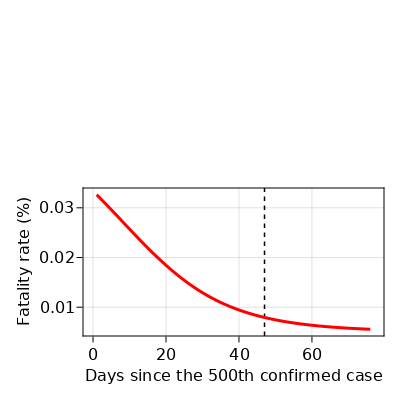
\includegraphics[width=\linewidth]{baseline/binhduong/20211216111951.baseline.binhduong.fatality_rate.png}
        \end{subfigure}
        \subcaption{Baseline model}
    \end{subfigure}

    \begin{subfigure}[b]{\linewidth}
        \centering
        \begin{subfigure}[b]{0.4\linewidth}
            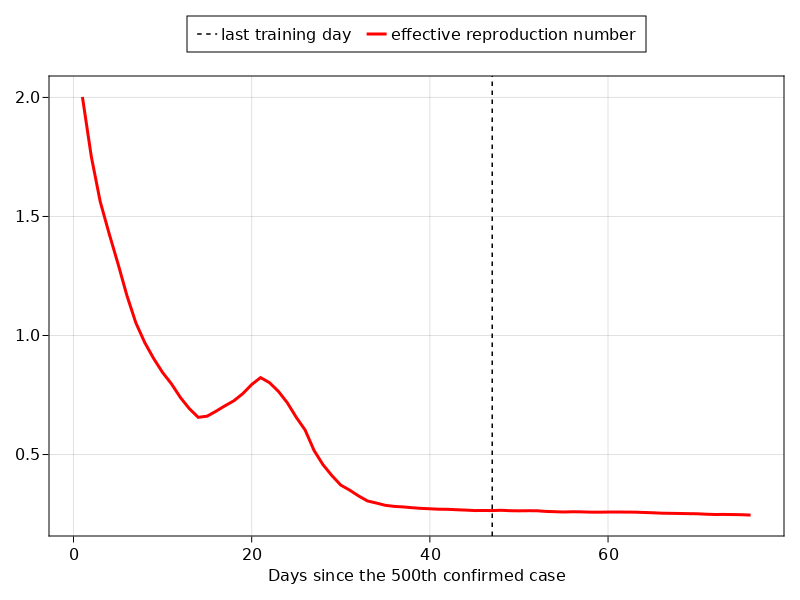
\includegraphics[width=\linewidth]{fb1/binhduong/20211216173307.fbmobility1.binhduong.R_effective.png}
        \end{subfigure}
        \begin{subfigure}[b]{0.4\linewidth}
            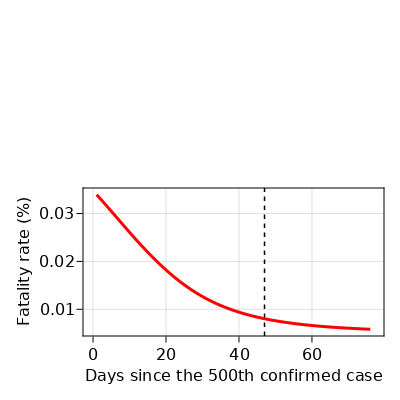
\includegraphics[width=\linewidth]{fb1/binhduong/20211216173307.fbmobility1.binhduong.fatality_rate.png}
        \end{subfigure}
        \subcaption{2nd. version}
    \end{subfigure}

    \begin{subfigure}[b]{\linewidth}
        \centering
        \begin{subfigure}[b]{0.4\linewidth}
            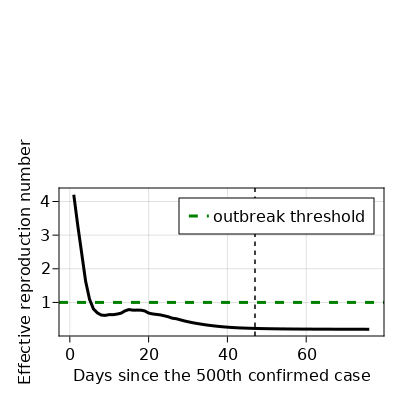
\includegraphics[width=\linewidth]{fb2/binhduong/20211216172741.fbmobility2.binhduong.R_effective.png}
        \end{subfigure}
        \begin{subfigure}[b]{0.4\linewidth}
            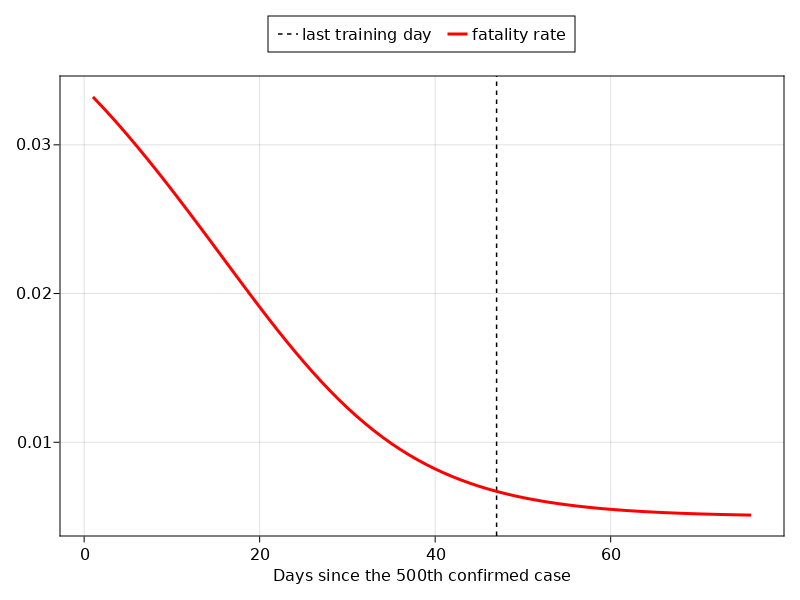
\includegraphics[width=\linewidth]{fb2/binhduong/20211216172741.fbmobility2.binhduong.fatality_rate.png}
        \end{subfigure}
        \subcaption{3rd. version}
    \end{subfigure}

    \caption{The effective reproduction number and the fatality rate for Binh Duong learned by different versions of the model}
    \label{fig:R0-and-fatality-binhduong}
\end{figure}

\begin{figure}[!htb]
    \centering

    \begin{subfigure}[b]{\linewidth}
        \centering
        \begin{subfigure}[b]{0.4\linewidth}
            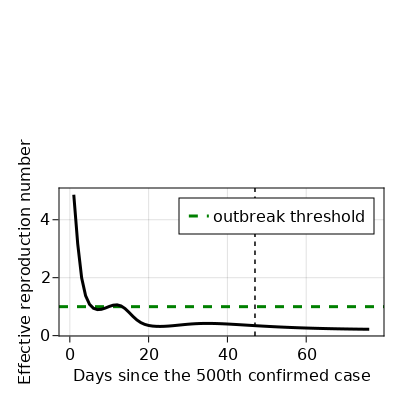
\includegraphics[width=\linewidth]{baseline/dongnai/20211216211601.baseline.dongnai.R_effective.png}
        \end{subfigure}
        \begin{subfigure}[b]{0.4\linewidth}
            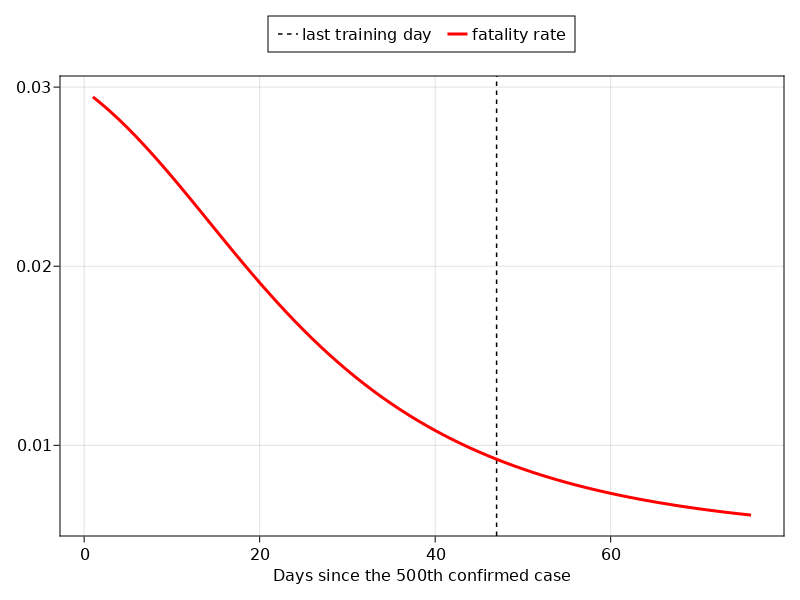
\includegraphics[width=\linewidth]{baseline/dongnai/20211216211601.baseline.dongnai.fatality_rate.png}
        \end{subfigure}
        \subcaption{Baseline model}
    \end{subfigure}

    \begin{subfigure}[b]{\linewidth}
        \centering
        \begin{subfigure}[b]{0.4\linewidth}
            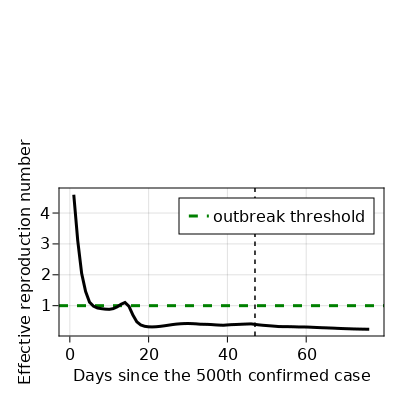
\includegraphics[width=\linewidth]{fb1/dongnai/20211216131821.fbmobility1.dongnai.R_effective.png}
        \end{subfigure}
        \begin{subfigure}[b]{0.4\linewidth}
            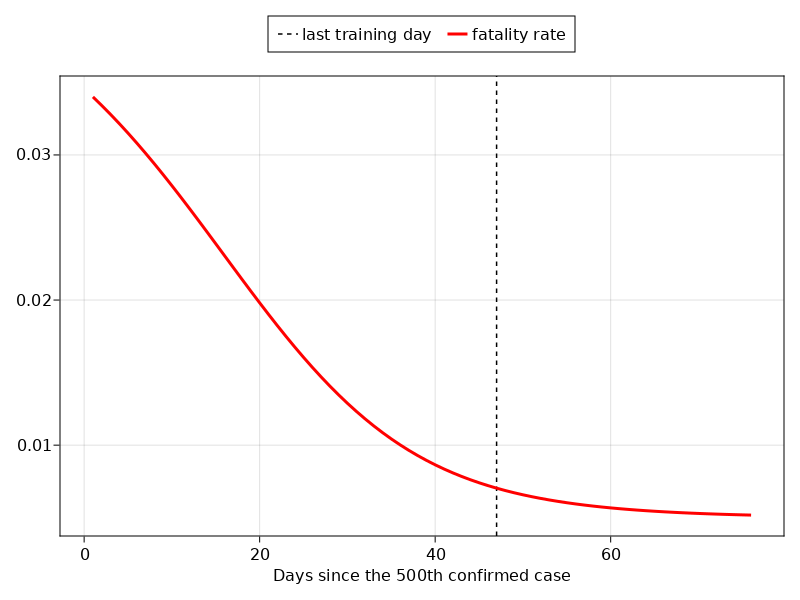
\includegraphics[width=\linewidth]{fb1/dongnai/20211216131821.fbmobility1.dongnai.fatality_rate.png}
        \end{subfigure}
        \subcaption{2nd. version}
    \end{subfigure}

    \begin{subfigure}[b]{\linewidth}
        \centering
        \begin{subfigure}[b]{0.4\linewidth}
            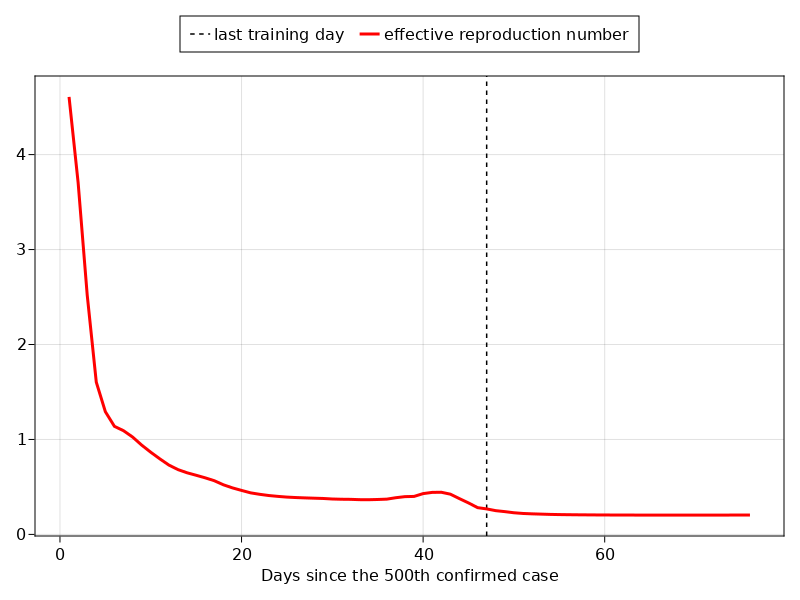
\includegraphics[width=\linewidth]{fb2/dongnai/20211217220549.fbmobility2.dongnai.R_effective.png}
        \end{subfigure}
        \begin{subfigure}[b]{0.4\linewidth}
            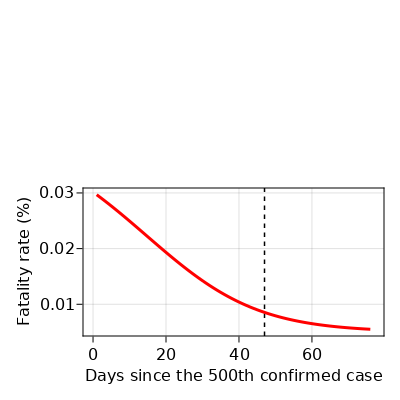
\includegraphics[width=\linewidth]{fb2/dongnai/20211217220549.fbmobility2.dongnai.fatality_rate.png}
        \end{subfigure}
        \subcaption{3rd. version}
    \end{subfigure}

    \caption{The effective reproduction number and the fatality rate for Dong Nai learned by different versions of the model}
    \label{fig:R0-and-fatality-dongnai}
\end{figure}


\begin{figure}[!htb]
    \centering

    \begin{subfigure}[b]{\linewidth}
        \centering
        \begin{subfigure}[b]{0.4\linewidth}
            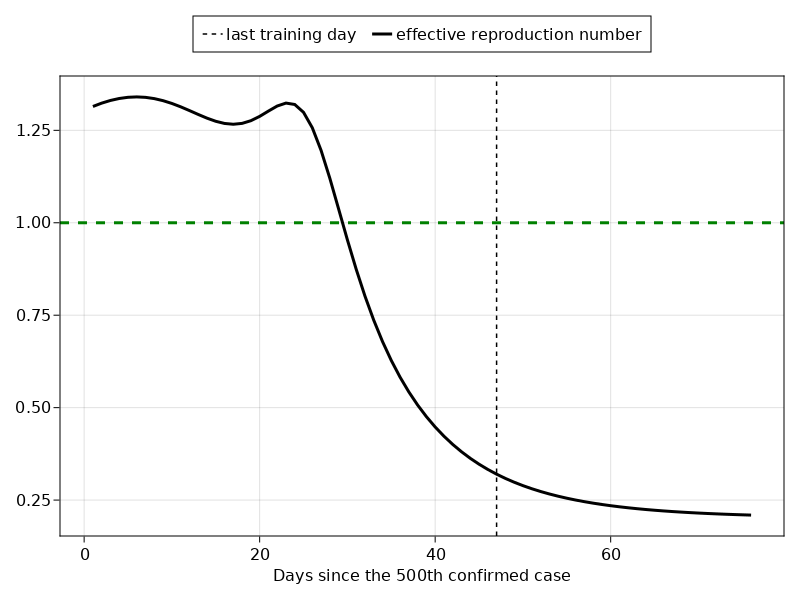
\includegraphics[width=\linewidth]{baseline/hcm/20211216154445.baseline.hcm.R_effective.png}
        \end{subfigure}
        \begin{subfigure}[b]{0.4\linewidth}
            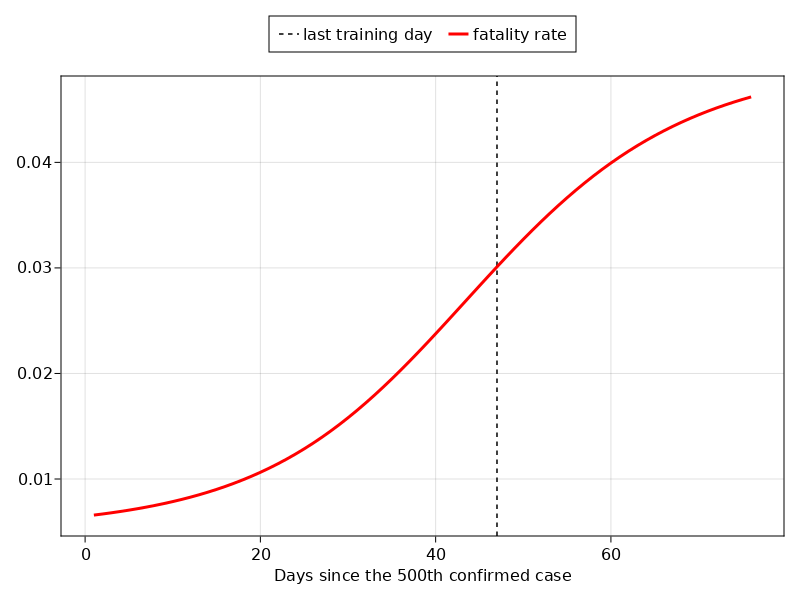
\includegraphics[width=\linewidth]{baseline/hcm/20211216154445.baseline.hcm.fatality_rate.png}
        \end{subfigure}
        \subcaption{Baseline model}
    \end{subfigure}

    \begin{subfigure}[b]{\linewidth}
        \centering
        \begin{subfigure}[b]{0.4\linewidth}
            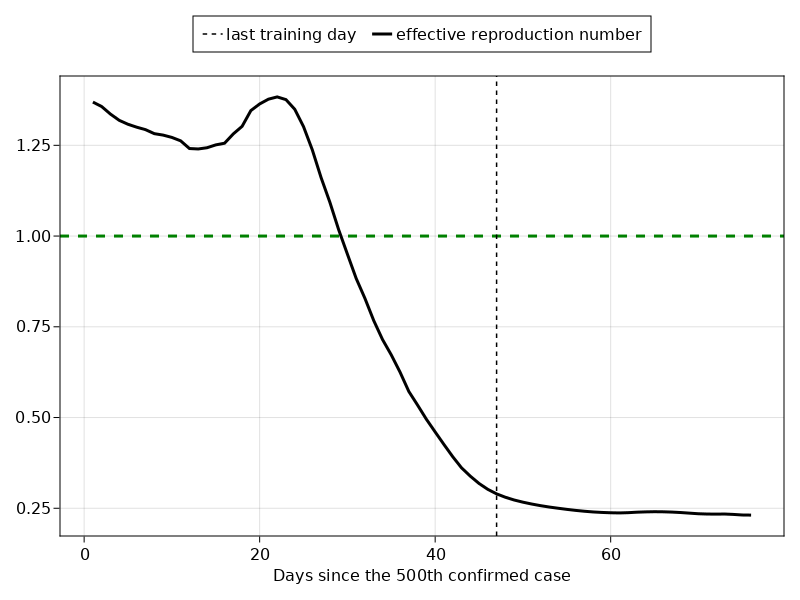
\includegraphics[width=\linewidth]{fb1/hcm/20211216231719.fbmobility1.hcm.R_effective.png}
        \end{subfigure}
        \begin{subfigure}[b]{0.4\linewidth}
            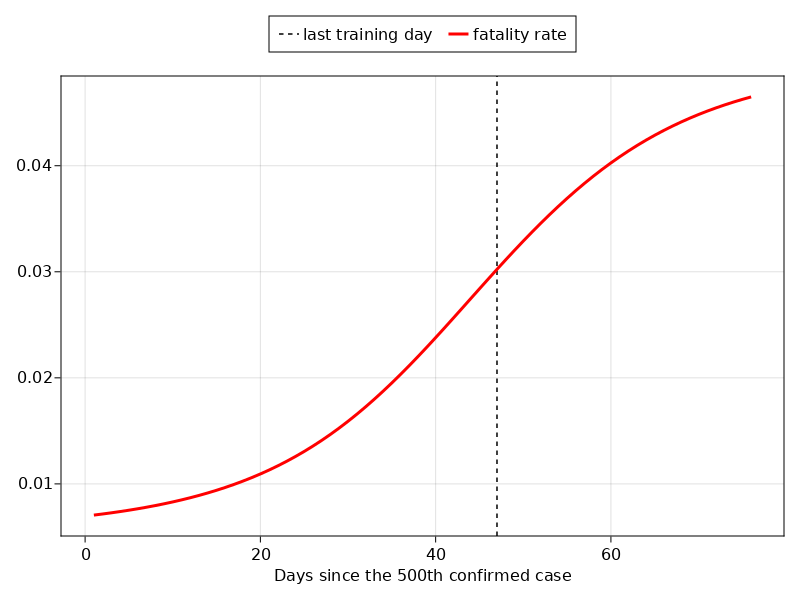
\includegraphics[width=\linewidth]{fb1/hcm/20211216231719.fbmobility1.hcm.fatality_rate.png}
        \end{subfigure}
        \subcaption{2nd. version}
    \end{subfigure}

    \begin{subfigure}[b]{\linewidth}
        \centering
        \begin{subfigure}[b]{0.4\linewidth}
            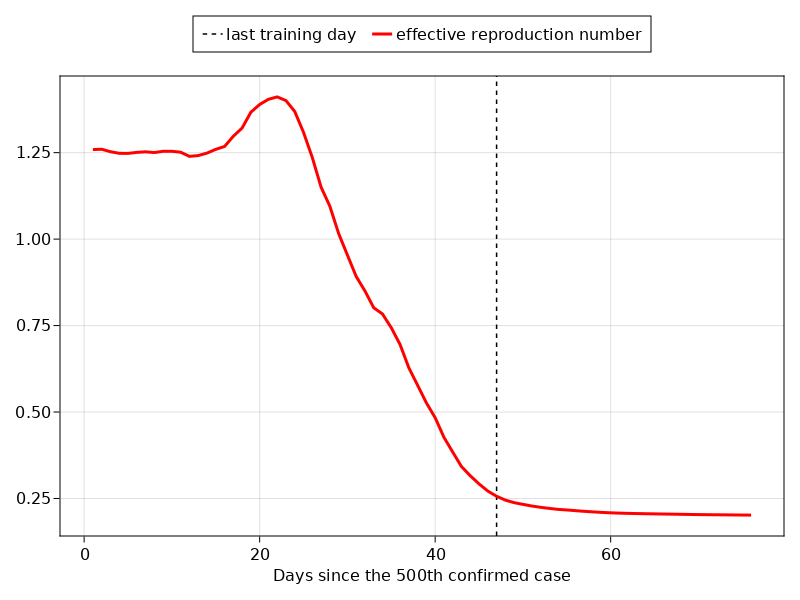
\includegraphics[width=\linewidth]{fb2/hcm/20211216183635.fbmobility2.hcm.R_effective.png}
        \end{subfigure}
        \begin{subfigure}[b]{0.4\linewidth}
            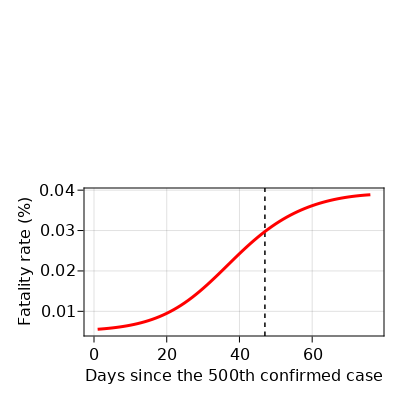
\includegraphics[width=\linewidth]{fb2/hcm/20211216183635.fbmobility2.hcm.fatality_rate.png}
        \end{subfigure}
        \subcaption{3rd. version}
    \end{subfigure}

    \caption{The effective reproduction number and the fatality rate for Ho Chi Minh city learned by different versions of the model}
    \label{fig:R0-and-fatality-hochiminh}
\end{figure}

\begin{figure}[!htb]
    \centering

    \begin{subfigure}[b]{\linewidth}
        \centering
        \begin{subfigure}[b]{0.4\linewidth}
            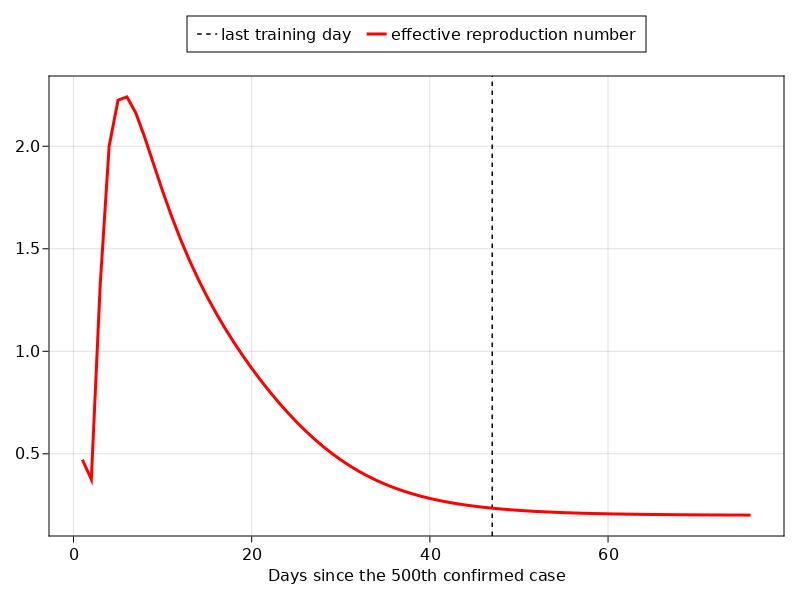
\includegraphics[width=\linewidth]{baseline/longan/20211216111951.baseline.longan.R_effective.png}
        \end{subfigure}
        \begin{subfigure}[b]{0.4\linewidth}
            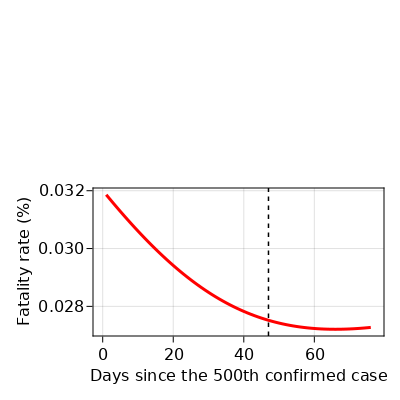
\includegraphics[width=\linewidth]{baseline/longan/20211216111951.baseline.longan.fatality_rate.png}
        \end{subfigure}
        \subcaption{Baseline model}
    \end{subfigure}

    \begin{subfigure}[b]{\linewidth}
        \centering
        \begin{subfigure}[b]{0.4\linewidth}
            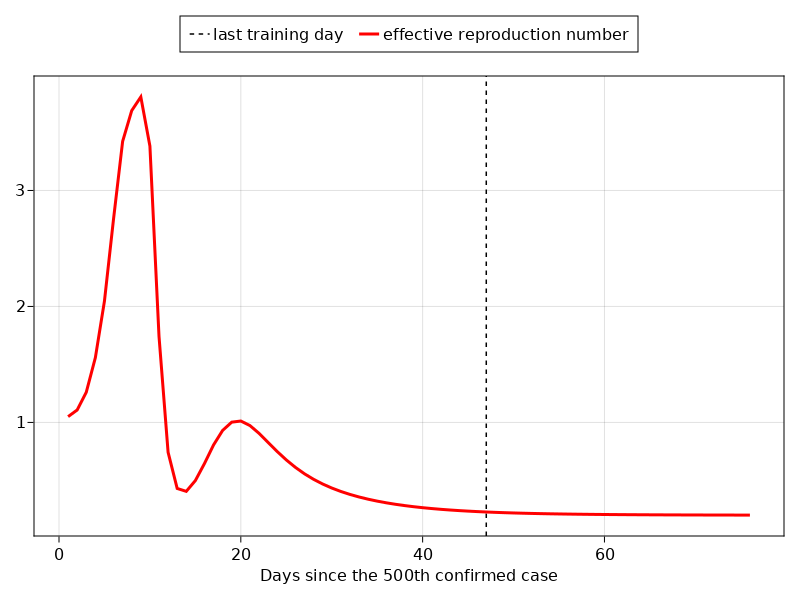
\includegraphics[width=\linewidth]{fb1/longan/20211216131821.fbmobility1.longan.R_effective.png}
        \end{subfigure}
        \begin{subfigure}[b]{0.4\linewidth}
            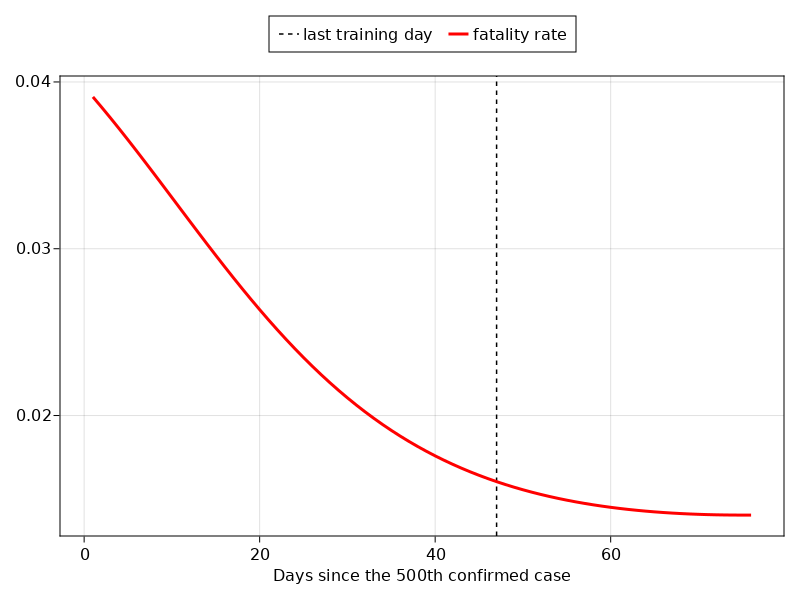
\includegraphics[width=\linewidth]{fb1/longan/20211216131821.fbmobility1.longan.fatality_rate.png}
        \end{subfigure}
        \subcaption{2nd. version}
    \end{subfigure}

    \begin{subfigure}[b]{\linewidth}
        \centering
        \begin{subfigure}[b]{0.4\linewidth}
            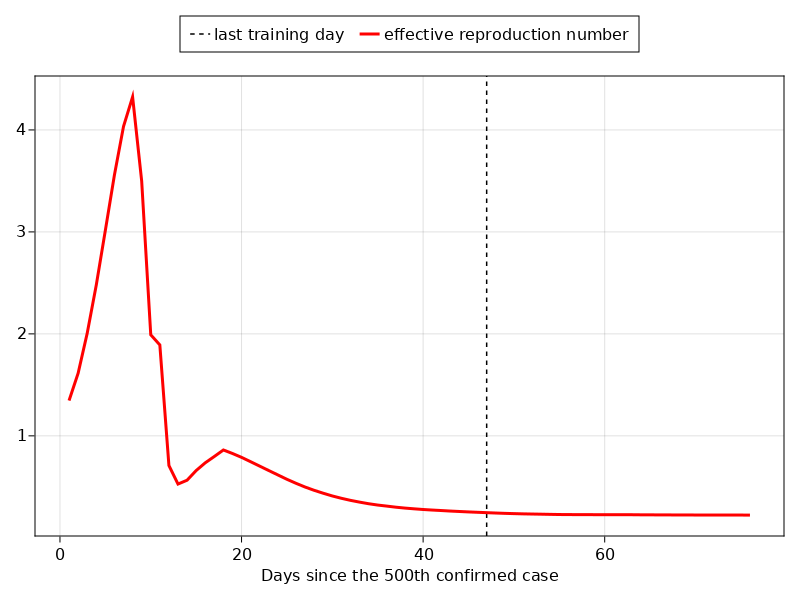
\includegraphics[width=\linewidth]{fb2/longan/20211216193717.fbmobility2.longan.R_effective.png}
        \end{subfigure}
        \begin{subfigure}[b]{0.4\linewidth}
            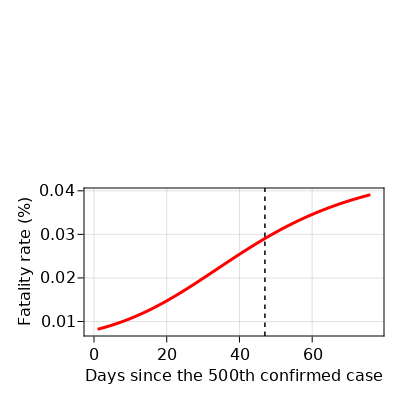
\includegraphics[width=\linewidth]{fb2/longan/20211216193717.fbmobility2.longan.fatality_rate.png}
        \end{subfigure}
        \subcaption{3rd. version}
    \end{subfigure}

    \caption{The effective reproduction number and the fatality rate for Long An learned by different versions of the model}
    \label{fig:R0-and-fatality-longan}
\end{figure}
